\setcounter{section}{3}
\section{Frequenzgang und Polstellenlage}
\begin{tcolorbox}[colback=white!10!white,
                  colframe=green!30!black,
                  title=Auswirkung der NST und Polstellenlage] 
    \begin{figure}[H]
        \centering
        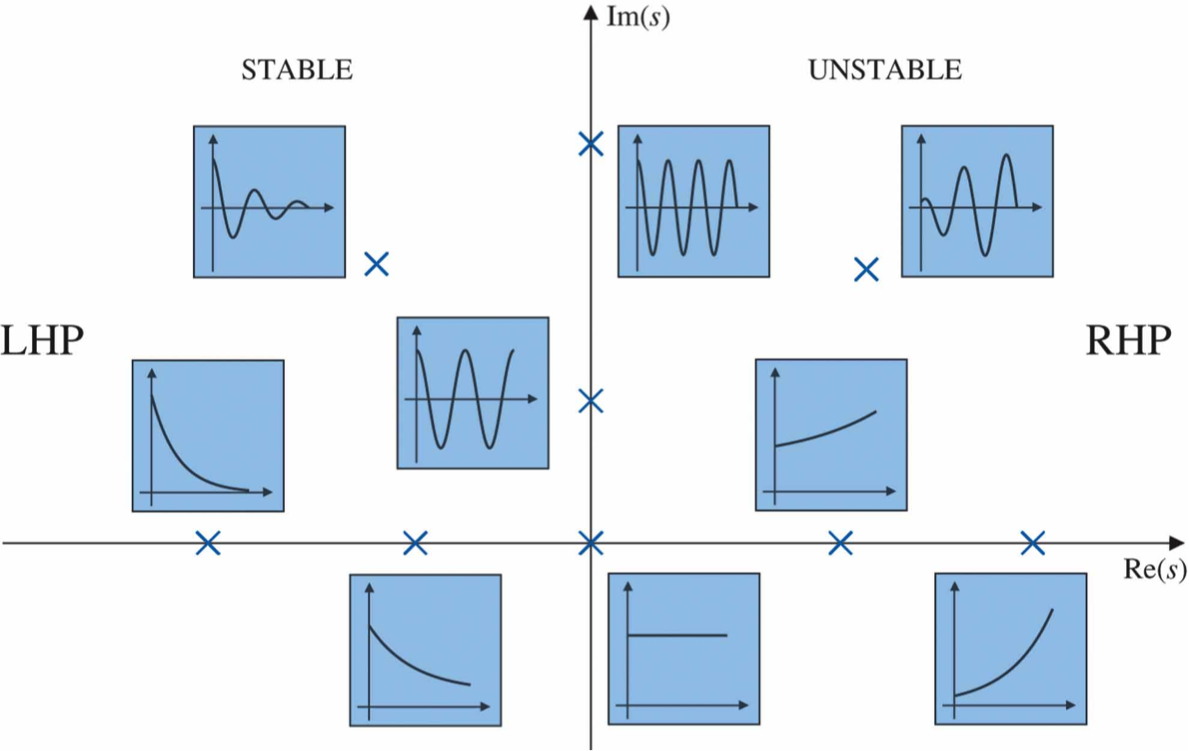
\includegraphics[width=1\textwidth]{images/lageAntwort}
    \end{figure}
    \tcblower
    \textbf{Polstelle (reell + komplexes Polpaar)}
    \begin{table}[H]
        \centering
        \begin{tabular}{ccc}
            \hline Re & Im & Auswirkung \\ 
            \hline $<$ 0 & = 0 & stabil - keine Schwingung \\ 
            \hline $>$ 0  & =0 & instabil - keine Schwingung \\ 
            \hline $=0$ & =0 & instabil - keine Schwingung \\ 
            \hline\hline $< 0$ & $\not =$ & stabil - Schwingung \\ 
            \hline $> 0$  &  $\not =$ & instabil - Schwingung \\ 
            \hline = 0  & $\not =$ & Dauerschwingung \\ 
            \hline 
        \end{tabular} 
    \end{table}
    \textbf{Nullstelle:}
    \begin{table}[H]
        \centering
        \begin{tabular}{p{2cm}p{3cm}}
            \hline $< = 0 $ & minimalphasiges System (evtl. Überschwung) \\ 
            \hline $> = 0 $ & nichtminimalphasiges System (Systemantwort erst entgegen der Sprunganregung) \\ 
            \hline $= 0 $ & $lim_{t\rightarrow\infty}y(t)\rightarrow 0$ \\ 
            \hline 
        \end{tabular} 
    \end{table}
\end{tcolorbox}

\subsection{PT$_2$ - Glied}
\begin{tcolorbox}[colback=white!10!white,
                  colframe=green!30!black,
                  title=PT$_2$ - Glied] 
    \begin{figure}[H]
        \begin{minipage}{.3\textwidth}
            \centering
            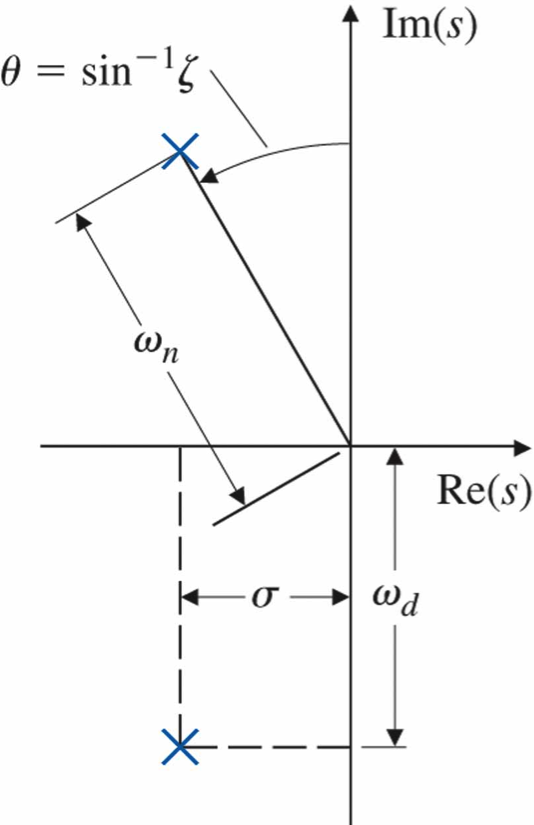
\includegraphics[width=1\textwidth]{images/winkel}
        \end{minipage}%
        \hspace{0.05\textwidth}
        \begin{minipage}{.65\textwidth}
            Instabilität beginnt in der rechten Halbebene. 
            
            Für die  \textbf{Dämpfung} gilt, je kleiner der Winkel $\theta$, 
            desto kleiner ist die Dämpfung:
            \begin{align*}
                \theta = \arcsin{\zeta}
            \end{align*}
            \textbf{Charakteristische Gleichung:} \\
            $a(s) = s^2 + 2\zeta\omega_ns + \omega_n^2
                  = \left(s+\sigma\right)^2 + \omega_d^2$
        \end{minipage}%
    \end{figure}
\end{tcolorbox}

\subsection{Kenngrößen im Zeitbereich}
\begin{tcolorbox}[colback=white!10!white,
                  colframe=green!30!black,
                  title=Kenngrößen] 
    \begin{figure}[H]
        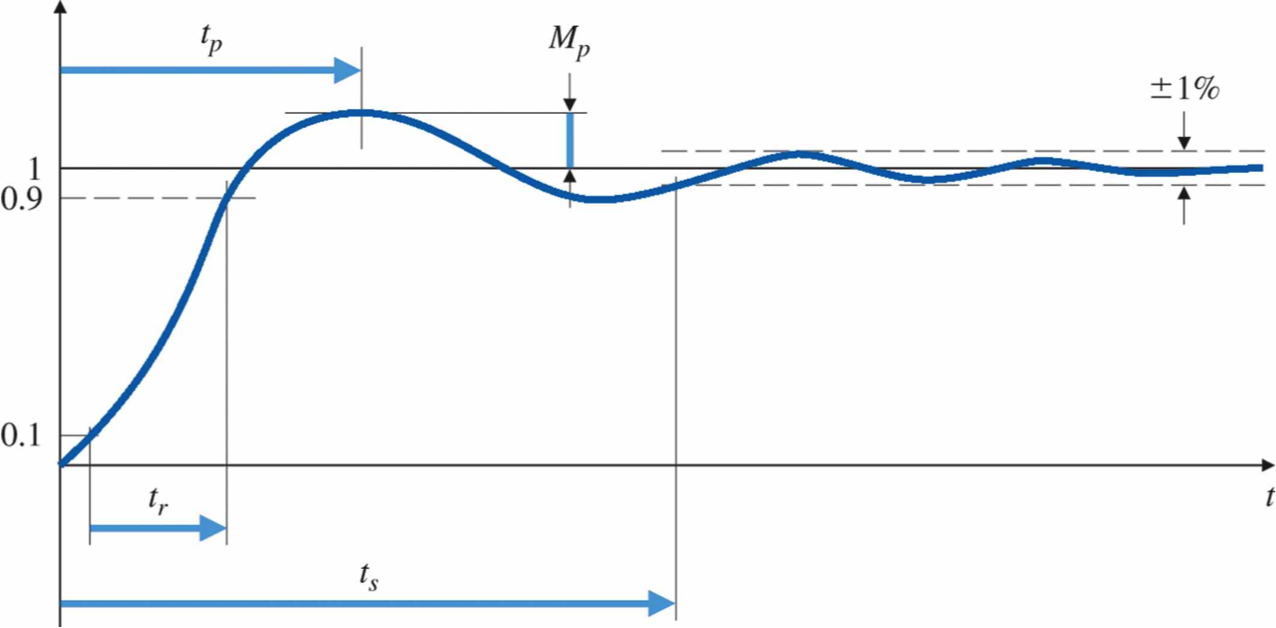
\includegraphics[width=1\linewidth]{images/numb}
    \end{figure}
    $\begin{matrix*}[l]
        \text{Steigzeit }[0.1, 0.9]\text{:}
            && \pm 1\%\text{-Einschwingzeit:} \\
        t_r \approx \frac{1,8}{\omega_n}
            && t_s = \frac{\ln{0.01}}{\zeta\omega_n} = \frac{4,6}{\sigma} \\\\
        \text{Überschwingweite:}
            && \text{Anstiegszeit:} \\
        M_p = e^{\frac{-\pi \zeta}{\sqrt{1-\zeta^2}}}
            && t_p = \frac{\pi}{\omega_n \sqrt{1-\zeta^2}} =\frac{\pi}{\omega_d} \\
            0 \leq \zeta \leq 1 \\\\
        \text{Gedämpfte Kreisfrequenz:}
            && \text{Ungedämpft zu gedämpft} \\
        \omega_d = \omega_n*\sqrt{1-\zeta^2}
            && \omega_n^2 = \sigma^2+\omega_d^2 \\
    \end{matrix*}$
    Dämpfung $\zeta = \sqrt{\frac{\ln(M_p)^2}{\pi^2+\ln(M_p)^2}}$
\end{tcolorbox}

